\documentclass[conference]{IEEEtran}
\usepackage{cite}
\usepackage{amsmath,amssymb,amsfonts}
\usepackage{graphicx}
\usepackage{textcomp}
\usepackage{xcolor}
\usepackage{booktabs}
\def\BibTeX{{\rm B\kern-.05em{\sc i\kern-.025em b}\kern-.08em
    T\kern-.1667em\lower.7ex\hbox{E}\kern-.125emX}}
\begin{document}

\title{Adaptive Study Planning for Self-Directed Learners: Context-Aware Pace Calibration with Change-Point Detection}

\author{
\IEEEauthorblockN{1\textsuperscript{st} Rohit Saji}
\IEEEauthorblockA{
\textit{Dept. of Data Science and Artificial Intelligence} \\
\textit{PES University} \\
Bengaluru, India \\
iam.rohitsaji@gmail.com}
\and
\IEEEauthorblockN{2\textsuperscript{nd} Ramesh Prakash Guledgudd}
\IEEEauthorblockA{
\textit{PES University} \\
Bengaluru, India \\
rameshpg1988@gmail.com}
}

\maketitle

\begin{abstract}
Self-directed study plans often become inaccurate after only a few logged sessions because the assumed pace is fixed at plan creation. This paper reports a local-first study-planning prototype and an offline component evaluation of its adaptation path. The prototype stores session events in the client, sends accumulated history to a Python service for pace calibration and shift detection, asks the learner to confirm a recalibration prompt, and projects finish dates in the client. The evaluation uses synthetic learner logs with planted ground truth, calibrated against OULAD engagement moments, across 200 seeds, 5{,}400 learners, and 346{,}394 sessions in the main frozen and decoupled regimes. The context-aware shrinkage calibrator reduced prospective pace-prediction error against the hierarchical-Bayesian incumbent in every decoupled-regime history band, with absolute reductions from 0.0145 to 0.0307 and Holm correction retained in all 12 tested cells. CUSUM gave low shift-detection latency but higher prompt burden. Projection results show that uncorrected Gaussian-process intervals under-cover, while split-conformal correction restores near-nominal coverage in research and remains outside the prototype. The results support component behavior under synthetic assumptions; they do not establish real-user learning-outcome gains.
\end{abstract}

\begin{IEEEkeywords}
adaptive learning, Bayesian calibration, change-point detection, Gaussian processes, study planning, self-regulated learning
\end{IEEEkeywords}

\section{Introduction}
Self-directed learners often translate an online course, certification target, or examination syllabus into a fixed calendar plan. The plan usually assumes a daily study duration, an estimated pace for each item, and a target completion date.

Those assumptions can become inaccurate early. A learner may miss a booking, complete a session faster than expected, or spend longer than planned on a difficult item. The displayed completion date then becomes a stale estimate, even though the learner's own log already contains evidence that the plan should be recalibrated.

Existing tools address only part of this problem. Time-tracking applications record study duration but do not maintain a plan. Static plan generators, including deep-learning-plus-optimization approaches such as that of Islam et al.~\cite{islam2024}, compute a schedule once from a predicted pace and do not revise it against the pace subsequently observed. The missing step is to use the learner's session history as evidence for plan revision while keeping the learner in control of the replan action.

The technical difficulty is that the evidence is sparse and non-stationary. A single learner produces only a few sessions before the first useful recalibration, so the model cannot rely on large per-learner samples. The same learner's pace can also shift when workload, time of day, or study conditions change. The system must therefore estimate pace under limited history and distinguish persistent shifts from ordinary variation before prompting a revision.

This paper makes the following contributions.
\begin{itemize}
\item A context-aware pace calibrator that augments hierarchical Bayes with 10 observable session features and population-prior shrinkage, evaluated against moving-average, EWMA, pooled-Bayes, and hierarchical-Bayes baselines.
\item A human-confirmed adaptation flow in an implemented local-first prototype: server-side pace calibration and single-arm CUSUM prompting, client-side progress projection, and capacity bookings that replace item-level day packing.
\item An offline comparison protocol over 200 seeds, held-out learner archetypes, bootstrap confidence intervals, and Holm/Benjamini--Hochberg correction, applied to calibration, detection, projection, and the retired packed-slot scheduler.
\item An implementation boundary that separates promoted prototype behavior from research results: the cold-start GP composite and enriched calibrator are promoted, while split-conformal interval correction and tuned dual-arm CUSUM remain future app work.
\end{itemize}

\section{Related Work}
Learner pace modeling draws on a broader learner-modeling literature in which Bayesian structure is used to control overfitting under sparse observations. Chen et al.~\cite{chen2024} present a hierarchical Bayesian model of adaptive teaching, validated across two behavioral experiments with 312 adults, showing how hierarchical priors capture learner-to-learner variability from limited evidence. Zambrano et al.~\cite{zambrano2024} examine Bayesian Knowledge Tracing and carelessness detectors at scale, while Mai et al.~\cite{mai2025} combine temporal modeling with a probabilistic layer to recover interpretable estimates. These studies motivate Bayesian calibration for learner models, but their targets are correctness, mastery, or bias analysis rather than planned-versus-actual study pace.

Change detection provides the second component needed for replanning. Saqr et al.~\cite{saqr2026} apply critical-slowing-down indicators to 1.67~million practice attempts from 9{,}401 students and report detectable warning signals before disengagement for 88.2\% of disengaging learners. Aminikhanghahi and Cook~\cite{aminikhanghahi2017} survey time-series change-point methods, and Roberts~\cite{roberts1959} gives the classical EWMA control-chart basis used in the detector comparison. These sources support statistical detection of behavioral shifts, but they do not specify how a study planner should expose the signal to the learner.

Progress projection is related to work on uncertainty-aware prediction from learning traces. P\'erez-Suay et al.~\cite{perezsuay2024} apply Gaussian-process regression with an automatic-relevance-determination kernel to learning-management-system logs and report a correlation of $R=0.89$ for predicting student marks. Lin et al.~\cite{lin2024} scale Gaussian processes to learning-curve prediction with a latent Kronecker structure, matching Transformer-level accuracy while retaining calibrated uncertainty. Split-conformal prediction gives a distribution-free method for repairing empirical interval coverage after fitting~\cite{angelopoulos2023}. The present work uses these ideas for finish-date projection rather than final-grade prediction.

Adaptive scheduling work provides the planning counterpart. Islam et al.~\cite{islam2024} couple an artificial neural network for grade prediction with dynamic programming for schedule optimization, establishing a predict-then-optimize pattern. In that setting, the schedule is solved from the predicted pace and is not revised against the learner's subsequent session history. This paper keeps the predict-then-optimize framing for evaluation, but studies what changes when observed pace is fed back into plan revision.

Self-regulated-learning analytics grounds the choice of schedule-related feedback signals. Alhazbi et al.~\cite{alhazbi2024} review 25 empirical studies measuring self-regulated learning from trace data and find that many validated indicators relate to time-management skill. de~Barba et al.~\cite{debarba2025} develop and validate a learning-analytics rubric that maps self-regulation scales onto learning-management-system indicators. These works support the use of trace-based time-management indicators, but they do not evaluate a local-first study planner that recalibrates its forecast from those traces.

Taken together, prior work supplies component methods for learner modeling, shift detection, projection, scheduling, and trace-based feedback. The narrower gap addressed here is their integration into one local-first study-planning prototype, with pace calibration, shift prompting, finish-date projection, and schedule redesign evaluated under the same synthetic ground-truth protocol.

\section{System Architecture}
\begin{figure*}[!t]
\centering
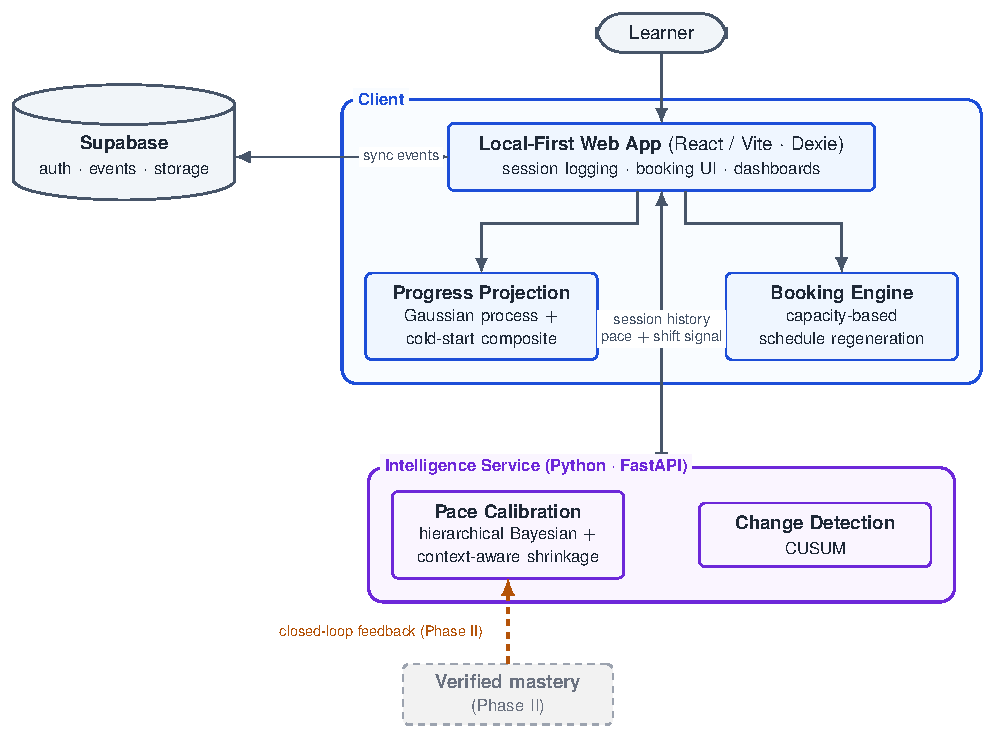
\includegraphics[width=0.8\textwidth]{fig_architecture.pdf}
\caption{Implemented prototype architecture. The client owns local event capture, booking interaction, the Gaussian-process plus analytic cold-start projection, and capacity bookings. The Python/FastAPI Intelligence Service fits the accumulated-history models used live: hierarchical Bayesian calibration with a context-aware shrinkage override and single-arm CUSUM prompting. Supabase supports authentication, persisted user data, and snapshots. Split-conformal interval correction and verified-mastery feedback are research or Phase-II work, not current prototype behavior.}
\label{fig:arch}
\end{figure*}
The implemented prototype is organized into two tiers of computation around a data hub. Computation that fits a statistical model to accumulated history runs on the server, while computation that derives a view directly from the learner's local event log runs on the client. Fig.~\ref{fig:arch} shows the resulting architecture.

The client is a local-first single-page application built with React and Vite, storing learner actions as events in a per-user IndexedDB store through Dexie. It owns the session-logging and booking interfaces, the dashboards, the Gaussian-process progress projection with its analytic cold-start fallback, and the capacity-based booking engine. Running these client-side keeps the core loop responsive and available offline. The Intelligence Service is a Python and FastAPI application that hosts pace calibration and change detection: on each request it receives the learner's session history over an authenticated HTTP call and returns a calibrated pace multiplier together with a change-detection signal. Every request carries a token issued at sign-in, which the service verifies before any model runs. Supabase sits between the client and the service as the data hub for authentication, persisted user data, and snapshots; the evaluation claims in this paper do not depend on real cloud user logs. The closed-loop feedback from a verified-mastery signal back into calibration, shown dashed in Fig.~\ref{fig:arch}, is the principal Phase-II extension and is not part of the implemented prototype.

This architecture follows a design revision. The starting point applied the predict-then-optimize architecture of Islam et al.~\cite{islam2024} directly: a predictive model estimated the learner's pace and a constraint-based optimizer packed each item of study material onto a specific calendar day, producing a dated slot grid that a replan re-computed in full. In the prototype this created concrete boundary cases. A missed booking, a partially completed item crossing a day boundary, or a small pace change could force many material assignments to move even when the learner only needed a new estimate of available study capacity. The scheduling question was therefore re-examined, and the prescriptive packer was replaced with the capacity-based booking model in Fig.~\ref{fig:arch}: the plan holds blank bookings, each carrying a date and a duration, and the learner chooses the specific material at the start of a session. The pace-calibration, change-detection, and projection models were confirmed to transfer to the revised design (Section~V), so the redesign changed how a plan is represented, not what is estimated about the learner.

\section{Methodology}
Each component was chosen by comparing candidate models offline against established baselines rather than by assumption, using the procedure of Section~\ref{sec:method-compare}. Table~\ref{tab:candidates} summarizes the candidates considered per component and the approach used in the implemented prototype.

\begin{table*}[!t]
\centering
\caption{Candidate models per component and the approach used in the implemented prototype.}
\label{tab:candidates}
\begin{tabular}{p{2.6cm} p{7.6cm} p{6.4cm}}
\toprule
\textbf{Component} & \textbf{Candidates compared} & \textbf{Approach used in the implemented prototype} \\
\midrule
Pace calibration & Moving average, EWMA, pooled Bayesian, hierarchical Bayesian, context-aware shrinkage & Hierarchical Bayesian posterior (Eq.~\eqref{eq:bayes-update}) refined by the context-aware shrinkage calibrator (Eq.~\eqref{eq:enriched}) \\
Change detection & CUSUM, EWMA control chart, critical slowing down, Page--Hinkley, Bayesian online change-point, ADWIN & CUSUM change-point detection (Eq.~\eqref{eq:cusum}); the fastest detector, feeding a human-confirmed recalibration prompt \\
Progress projection & Linear extrapolation, Gaussian process, GP with cold-start composite, split-conformal interval correction & Gaussian process (Eq.~\eqref{eq:gp-kernel}) with a cold-start analytic composite; split-conformal correction is evaluated but not yet promoted \\
Schedule generation & Rule-based, dynamic-programming capacity allocator (Eq.~\eqref{eq:dp}), greedy prerequisite-aware, local-search repair & Not adopted; day-by-day packing was replaced by the capacity-based booking model of Section~III following the evaluation in Section~\ref{sec:res-sched} \\
\bottomrule
\end{tabular}
\end{table*}

\subsection{Pace Calibration}
\label{sec:method-cal}
For a session $t$, let the pace ratio be $r_t = a_t/p_t$, the ratio of active minutes $a_t$ to planned minutes $p_t$, modeled as $r_t \sim \mathcal{N}(\mu,\sigma^2)$ with prior $\mu \sim \mathcal{N}(\mu_0,\tau_0^2)$ centered at $\mu_0=1$. With $n$ observed sessions the conjugate posterior is Gaussian,
\begin{equation}
\begin{split}
p(\mu \mid r_{1:n}) &= \mathcal{N}(\mu_n,\tau_n^2), \\
\tau_n^2 &= \Big(\tfrac{1}{\tau_0^2}+\tfrac{n}{\sigma^2}\Big)^{-1}, \\
\mu_n &= \tau_n^2\Big(\tfrac{\mu_0}{\tau_0^2}+\tfrac{1}{\sigma^2}\sum_{t=1}^{n} r_t\Big).
\end{split}
\label{eq:bayes-update}
\end{equation}
This hierarchical Bayesian posterior is the incumbent: it stays close to the prior while $n$ is small, which is what makes a usable estimate available from a handful of sessions, and tightens around the learner's realized rate as $n$ grows.

The implemented service refines this estimate with a context-aware shrinkage calibrator. Let $\phi_t \in \mathbb{R}^d$ be a vector of observable session context, covering intercept, anchor role, practice role, morning, evening, weekend, same-day extra session, planned progress, deadline urgency, and recency, and let $y_t = \log(a_t/p_t)$ be the log pace ratio. The calibrator fits weights $w$ by ridge-regularized least squares shrunk toward a population prior $w_0$ rather than toward zero,
\begin{equation}
\hat{w} = \arg\min_{w}\ \sum_t \big(y_t - w^{\top}\phi_t\big)^2 \; + \; \lambda\,\lVert w \rVert^2 \; + \; \gamma\,\lVert w - w_0 \rVert^2,
\label{eq:enriched}
\end{equation}
with ridge strength $\lambda=2.0$ and population-prior shrinkage strength $\gamma=6.0$ in the promoted implementation. The pace multiplier for a context $\phi$ is $\exp(\hat{w}^{\top}\phi)$. Shrinking toward a population prior, rather than toward zero, lets the model behave sensibly when a learner has logged few sessions and converge to learner-specific behavior as sessions accumulate. The service refits the model on each calibration request rather than persisting model state. The promoted calibrator is an ensemble of two such models, seeded with different population priors and combined by leave-one-out-weighted averaging, with fixed fallback weights when fewer than two sessions are available.

\subsection{Change Detection}
\label{sec:method-det}
A one-sided cumulative-sum chart tracks the running deviation of the pace signal $x_t$ from its in-control mean $\mu_0$,
\begin{equation}
S_0 = 0, \qquad S_t = \max\!\big(0,\; S_{t-1} + (x_t-\mu_0) - k\big),
\label{eq:cusum}
\end{equation}
and the chart raises an alarm once $S_t > h$, where the slack $k$ absorbs ordinary day-to-day variation and $h$ is the decision threshold~\cite{aminikhanghahi2017}. The statistic stays near zero while the pace is stable and accumulates once a persistent shift occurs. A detected shift raises a recalibration prompt; the learner confirms or dismisses the prompt before any replan action (Section~\ref{sec:res-det}).

\subsection{Progress Projection}
\label{sec:method-proj}
A Gaussian process places a prior over progress curves and conditions it on the observed cumulative-progress points, under a squared-exponential kernel with signal variance $\sigma_f^2$ and length scale $\ell$,
\begin{equation}
k(x,x') = \sigma_f^2 \exp\!\Big(-\tfrac{(x-x')^2}{2\ell^2}\Big).
\label{eq:gp-kernel}
\end{equation}
The resulting predictive variance supplies an interval around the projected completion date, rather than a single point. The implemented client projection uses this Gaussian process with a cold-start composite: while fewer than five sessions have accumulated, or when the fitted GP would cross implausibly, it falls back to an analytic required-rate estimate. A split-conformal correction of the interval width is evaluated in Section~\ref{sec:res-proj}; it restores nominal coverage in research but is not yet part of the client implementation.

\subsection{Schedule Generation}
\label{sec:method-sched}
Writing $V(t,\rho)$ for the best achievable cost from day $t$ onward with remaining work $\rho$, a day-by-day scheduler solves a recurrence of the form
\begin{equation}
V(t,\rho) = \min_{0 \le a \le c_t}\ \big[\, \ell(a) + V(t+1,\ \rho - a)\,\big],
\label{eq:dp}
\end{equation}
where $a$ is the study time allocated on day $t$, $c_t$ is that day's capacity, and $\ell$ penalizes deadline drift~\cite{islam2024}. Section~\ref{sec:res-sched} reports that this allocator minimizes deadline drift among the scheduling candidates; Section~III records why the implemented prototype does not use it, replacing day-by-day packing with the capacity-based booking model instead.

\subsection{Offline Evaluation Dataset}
\label{sec:method-data}
The offline evaluation uses synthetic learner logs because the target quantities are not directly observable in real usage. Planted ground truth supplies each learner's pace, change schedule, and finish date, making pace recovery, detection latency, and interval coverage measurable. The synthetic generator was calibrated against Open University Learning Analytics Dataset (OULAD) engagement moments by aggregating \emph{studentVle.sum\_click} by learner, course, and day. OULAD was used as a bounded proxy for engagement intensity, not as direct validation of this prototype. The calibration pass saw 10{,}655{,}280 OULAD rows, retained 571{,}356 after filtering, and produced 1{,}440 usable learner-course series.

The main algorithm comparisons use two 5{,}400-learner regimes: a frozen anchor and a decoupled regime that models the later booking design with ad-hoc and interrupted sessions. Both contain 200 seeds, 9 learner archetypes, 3 history bands, and 346{,}394 generated sessions. The scheduling comparison uses an earlier 3{,}600-learner reality-matched regime because the packed-slot scheduling question was retired before the decoupled booking regime existed. Table~\ref{tab:eval-config} summarizes the stamped configuration.

\begin{figure}[!t]
\centering
\scriptsize
\begin{tabular}{@{}r p{0.86\linewidth}@{}}
1 & For each seed, history band, and learner archetype, draw the target session count and material mix. \\
2 & Draw study days, ad-hoc bookings, interruption targets, and learner adherence bias for the decoupled regime. \\
3 & Build dated bookings, assign material chunks, and mark completed or interrupted session resolutions. \\
4 & Plant latent pace from global, role, time-of-day, weekend, fatigue, deadline, trend, and step/drift regime multipliers. \\
5 & Emit active or manual session events with planned minutes, active minutes, material role, progress position, booking id, and source. \\
6 & Write learner JSONL plus sidecar ground truth containing pace sequence, regime schedule, finish date, and manifest hashes. \\
\end{tabular}
\caption{Synthetic generator pseudocode for the decoupled regime used in the main calibration, detection, and projection results.}
\label{fig:synthetic-generator}
\end{figure}

\begin{table}[!t]
\centering
\caption{Main synthetic-generator parameters used in the frozen and decoupled regimes.}
\label{tab:generator-params}
\scriptsize
\begin{tabular}{p{2.55cm} p{4.45cm}}
\toprule
\textbf{Parameter} & \textbf{Value} \\
\midrule
Archetypes & steady, morning lark, fading flame, weekend warrior, deadline sprinter, marathon runner, night owl, crammer, steady improver \\
History bands & small 8--20 sessions, medium 35--70 sessions, max 90--160 sessions \\
Pace ratio bounds & $r_t = a_t/p_t$ clipped to $[0.55,1.60]$ \\
Noise model & lognormal AR(1), $\phi=0.30$, archetype-specific $\sigma_{\log}=0.15$--0.25 \\
Role/time multipliers & anchor 1.10, foundation 1.00, practice 0.92; generic morning 0.97, afternoon 1.00, evening 1.05 \\
Shift planting & step magnitude sampled from 0.10--0.22; drift total 0.20 over 30\%--45\% of sessions \\
Decoupled design & study days 3--6 per week; ad-hoc target 10\%--20\%; interruption target 15\%--25\%; adherence bias clipped to 0.85--1.20 \\
Manifest note & frozen hash 21c2cdabfa91; decoupled dataset synthetic-decoupled-9e6d48db2da8-seed0-n5400 with decoupled parameter hash a99216b83551 \\
\bottomrule
\end{tabular}
\end{table}

\begin{table}[!t]
\centering
\caption{Offline evaluation configuration extracted from result manifests and synthetic JSONL files.}
\label{tab:eval-config}
\scriptsize
\begin{tabular}{p{2.45cm} p{4.55cm}}
\toprule
\textbf{Item} & \textbf{Value} \\
\midrule
Main regimes & Frozen and decoupled, each with 200 seeds, 5{,}400 learners, and 346{,}394 sessions \\
Scheduling regime & Reality-matched packed-slot regime, 200 seeds, 3{,}600 learners, and 230{,}469 sessions \\
History bands & Small, medium, and max; generated sessions per learner have min/median/max 8/53/160 \\
Archetypes & 9 for calibration, detection, and projection; 6 for scheduling \\
Held-out protocol & 5 train archetypes and 4 held-out archetypes; scoring uses the held-out split \\
Decoupled events & 51{,}813 ad-hoc sessions and 69{,}436 interrupted sessions \\
OULAD moment bounds & Gap days p50/p75/p90/p95 = 1/3/6/11; dropout probability range 0.140--0.290; shift frequency range 0.25--20 per 100 days \\
Corrections & Learner-level bootstrap delta intervals; Holm-Bonferroni primary correction; Benjamini--Hochberg reported \\
Oracle & Uses planted ground truth as an upper-bound reference; not a deployable method \\
\bottomrule
\end{tabular}
\end{table}

\subsection{Comparison Methodology}
\label{sec:method-compare}
Each candidate was evaluated offline on the datasets summarized in Table~\ref{tab:eval-config}. Candidates were evaluated on held-out learner archetypes absent from the set used to develop them, so that a win reflects generalization rather than fitting to the evaluation cases. Every reported comparison carries a bootstrap confidence interval on the difference between a candidate and the incumbent, estimated by resampling learners with replacement, and a Holm or Benjamini--Hochberg correction is applied across the family of comparisons. An oracle baseline, given the planted ground truth, is included in the results that follow as an upper-bound reference; it is never treated as a deployable method.

\section{Results and Discussion}
All results below are computed on the synthetic ground-truth datasets described in Section~\ref{sec:method-data}. Calibration and projection are reported for both the frozen synthetic regime and the decoupled regime that matches the capacity-based booking model, so that transfer across the redesign can be checked. Scheduling is reported only for the earlier packed-slot regime, since the scheduling formulation was retired before the decoupled booking regime existed. Throughout, the oracle is an upper-bound reference given the planted ground truth; it is never treated as a deployable method.

\subsection{Pace Calibration}
\label{sec:res-cal}
Two calibration metrics were separated. Recovery error measures how closely an estimate reconstructs the planted pace after the fact. Prospective context-prediction error measures the next-session pace estimate used by the planner. On recovery error, no structured Bayesian candidate consistently improves over the hierarchical-Bayesian incumbent, and the incumbent remains strongest among deployable methods at the longest histories. On prospective context prediction, the context-aware shrinkage calibrator improves over the incumbent across every history-length band and across both synthetic regimes (Table~\ref{tab:res-cal}). Because the planner must act before much learner history is available, this prospective metric determined the promoted calibration path.

\begin{table}[!t]
\centering
\caption{Shrinkage minus hierarchical-Bayesian prospective error; negative favors shrinkage.}
\label{tab:res-cal}
\scriptsize
\begin{tabular}{@{}l c c@{}}
\toprule
\textbf{Band} & \textbf{Frozen $\Delta$} & \textbf{Decoupled $\Delta$} \\
\midrule
Short & $-0.0148$ [$-0.0168,-0.0127$] & $-0.0145$ [$-0.0155,-0.0136$] \\
Medium & $-0.0262$ [$-0.0282,-0.0243$] & $-0.0268$ [$-0.0277,-0.0258$] \\
Long & $-0.0300$ [$-0.0316,-0.0285$] & $-0.0307$ [$-0.0316,-0.0299$] \\
\bottomrule
\end{tabular}
\end{table}

Table~\ref{tab:res-cal-ablation} expands the calibration comparison into an ablation-style view for the decoupled regime. It should be read as a candidate-family comparison, not a strict causal ablation, because some rows change more than one design choice at once. The main pattern is that context features matter: context-aware rows reduce prospective error relative to SMA, EWMA, pooled Bayes, and hierarchical Bayes in all three bands.

The promotion rule was not the lowest value in a single table. A candidate had to improve held-out prospective prediction, avoid an unacceptable recovery-error regression in the frozen and earlier reality-matched checks, transfer across the booking redesign, and fit the prototype's stateless request/response service. The empirical-Bayes partial-pooling row is lowest on the decoupled prospective means, but it failed those broader recovery and transfer guardrails. It is therefore reported as a research finding, while the \textit{enriched\_shrink}/dual-prior path remains the promoted app model.

\begin{table}[!t]
\centering
\caption{Decoupled-regime ablation-style comparison for prospective context-prediction error. Lower is better; design abbreviates context and prior choices.}
\label{tab:res-cal-ablation}
\scriptsize
\begin{tabular}{@{}l l r r r@{}}
\toprule
\textbf{Candidate} & \textbf{Design} & \textbf{Short} & \textbf{Med.} & \textbf{Long} \\
\midrule
SMA & no context & 0.07070 & 0.06258 & 0.05831 \\
EWMA & prior start & 0.07083 & 0.06320 & 0.06076 \\
Pooled Bayes & pooled prior & 0.07099 & 0.06772 & 0.06378 \\
Hier. Bayes & incumbent & 0.07099 & 0.06772 & 0.06378 \\
Cov. Bayes & ridge context & 0.05422 & 0.03740 & 0.02780 \\
EB partial & grouped context & 0.03636 & 0.02258 & 0.01512 \\
Enriched & 10-feature prior & 0.05646 & 0.04096 & 0.03307 \\
Dual prior & 10-feature ens. & 0.05646 & 0.04096 & 0.03307 \\
\bottomrule
\end{tabular}
\end{table}

\subsection{Change Detection}
\label{sec:res-det}
Table~\ref{tab:res-det} reports the decoupled-regime detector comparison. CUSUM has the lowest latency on both step and drift shifts and wins the selection score in this regime, but it also produces more false alarms than CSD, EWMA, BOCPD, or ADWIN. As a prompt-burden metric, the selected CUSUM averages 10.68 false alarms per held-out learner-run, with a 90th percentile of 22, equivalent to about 1.92 false prompts per 10 observations. This trade-off is acceptable only because the prototype raises a prompt rather than automatically changing the plan; a false alarm can be dismissed, but frequent prompts would still need throttling or tuning in real use. The implemented detector is a simpler single-arm CUSUM; the benchmark's tuned dual-arm CUSUM is future promotion work.

\begin{table}[!t]
\centering
\caption{Decoupled-regime change-detection results. False alarms are rates; lower latency and score are better.}
\label{tab:res-det}
\scriptsize
\begin{tabular}{@{}l l r r r r@{}}
\toprule
\textbf{Detector} & \textbf{Shift} & \textbf{Lat.} & \textbf{FA} & \textbf{Miss} & \textbf{Score} \\
\midrule
ADWIN & Step & $\infty$ & 0.000 & 200 & $\infty$ \\
ADWIN & Drift & $\infty$ & 0.000 & 600 & $\infty$ \\
BOCPD & Step & 13.052 & 0.005 & 142 & 14213.2 \\
BOCPD & Drift & 8.746 & 0.006 & 123 & 12308.9 \\
CSD & Step & 4.670 & 0.049 & 3 & 305.9 \\
CSD & Drift & 5.320 & 0.033 & 166 & 16606.1 \\
CUSUM & Step & 1.375 & 0.180 & 0 & 5.9 \\
CUSUM & Drift & 2.294 & 0.192 & 2 & 207.1 \\
EWMA & Step & 6.317 & 0.030 & 20 & 2007.1 \\
EWMA & Drift & 7.007 & 0.031 & 66 & 6607.8 \\
Page--H. & Step & 3.055 & 0.138 & 0 & 6.5 \\
Page--H. & Drift & 2.500 & 0.125 & 42 & 4205.6 \\
\bottomrule
\end{tabular}
\end{table}

\subsection{Progress Projection}
\label{sec:res-proj}
The raw Gaussian-process interval under-covers: against a nominal 95\% coverage, the plain interval covers only 18\% to 49\% of cases depending on the history-length band in the decoupled regime (Table~\ref{tab:res-proj}). The cold-start composite improves the small-band point estimate and is the projection refinement currently implemented in the client. The split-conformal correction addresses a different failure mode: it widens the interval to restore near-nominal coverage while leaving the point estimate unchanged. In the decoupled regime it restores coverage to roughly 98.8\%--98.9\%, but the interval widths are large: 29.4 days for small histories, 119.4 for medium histories, and 292.3 for long histories. The corrected interval is therefore better suited to conservative internal risk assessment than to immediate user-facing completion-date display.

\begin{table}[!t]
\centering
\caption{Decoupled-regime projection results. Width is interval sharpness in days; nominal coverage is 0.95.}
\label{tab:res-proj}
\scriptsize
\begin{tabular}{@{}l l r r r@{}}
\toprule
\textbf{Method} & \textbf{Band} & \textbf{Cov.} & \textbf{MAE} & \textbf{Width} \\
\midrule
Plain GP & Short & 0.494 & 2.361 & 1.649 \\
Plain GP & Medium & 0.277 & 15.331 & 4.715 \\
Plain GP & Long & 0.183 & 39.530 & 7.955 \\
Cold start & Short & 0.552 & 2.139 & 2.278 \\
Cold start & Medium & 0.291 & 17.099 & 6.222 \\
Cold start & Long & 0.195 & 52.105 & 10.707 \\
Conformal & Short & 0.989 & 2.361 & 29.408 \\
Conformal & Medium & 0.988 & 15.331 & 119.444 \\
Conformal & Long & 0.988 & 39.530 & 292.293 \\
\bottomrule
\end{tabular}
\end{table}

\subsection{Schedule Generation}
\label{sec:res-sched}
Among the packed-slot scheduling candidates, the dynamic-programming capacity allocator of Eq.~\eqref{eq:dp} minimizes deadline drift in every material mix tested. Its margin over a greedy incumbent grows as more material roles are interleaved: on the all-roles mix, the greedy incumbent drifts by 38.975 days while the dynamic-programming allocator drifts by 8.297 days, a difference of $-30.9$ days [$-31.7,-30.2$] under a 95\% bootstrap interval. The simpler anchor-only case is much closer, 3.113 days for greedy versus 1.732 for dynamic programming. This is a result for the retired packed-slot formulation, not behavior of the current prototype. As Section~III records, the day-by-day packing formulation these schedulers share was replaced by the capacity-based booking model before the revised synthetic regime existed; the comparison is therefore reported as an evaluated result that informed a design decision.

\subsection{Discussion}
\label{sec:res-discuss}
The evaluation changed how the prototype uses evidence. Retrospective recovery remains useful for diagnosis because it asks whether a model reconstructs the planted pace after observing history. The planner, however, acts on the next estimate it shows the learner. The prospective improvement in Table~\ref{tab:res-cal} is therefore most relevant in the small-history setting, where the plan has the least evidence and an early correction is most likely to matter.

The detector result points in a different direction. Low CUSUM latency is desirable only if the system can absorb false alarms without taking automatic action. The current prototype does this by requiring confirmation before replanning, but the false-prompt counts in Section~\ref{sec:res-det} indicate that confirmation alone is not enough; a deployed prompt flow would also need throttling, cooldowns, or stronger tuning.

The projection and scheduling results define separate boundaries. For projection, the point-estimate path is usable in the client, but the uncorrected interval should not be described as calibrated. For scheduling, the dynamic-programming result is valid within the retired packed-slot formulation, while the current product uses blank capacity bookings to avoid brittle item-level reassignment. These are design constraints, not only statistical outcomes.

Two findings appear in both the frozen and decoupled regimes: the prospective calibration improvement and the projection coverage shortfall. That cross-regime agreement supports the component claims under controlled assumptions. It does not establish that the prototype improves study outcomes for real learners.

\subsection{Limitations}
\label{sec:limitations}
The offline evaluation is useful because planted ground truth makes pace recovery, shift latency, and interval coverage measurable. However, synthetic results demonstrate behavior under controlled assumptions; they do not prove effectiveness for real learners. Real learner logs may include multitasking, inaccurate self-reports, missing sessions, changing motivation, and interruptions not fully represented by the generator.

The current prototype adapts to logged study behavior, not verified learning. Logged time is not equivalent to mastery. Phase~II verified-mastery feedback is therefore a required extension before the system can claim to adapt to learning rather than to study-time traces alone.

The implementation boundary is also important. The promoted prototype includes the enriched pace calibrator, single-arm CUSUM prompting, the GP plus analytic cold-start projection, and capacity bookings. The split-conformal interval correction and tuned dual-arm CUSUM are evaluated research findings, but they remain future app-promotion work.

\section{Conclusion and Future Work}
This paper presented a local-first adaptive study-planning prototype in which logged study events are used to recalibrate a learner's plan. The implemented system combines client-side event storage and finish-date projection with server-side pace calibration and shift detection, and it keeps replanning under learner confirmation rather than automatic policy action.

The component evaluation showed that the main calibration benefit comes from prospective short-history prediction rather than retrospective recovery. It also identified constraints on the other adaptive components: fast shift detection must be balanced against prompt burden, and Gaussian-process finish-date intervals require calibration before they can be presented as reliable uncertainty estimates. The scheduling experiment contributed a design lesson rather than a promoted algorithm: dynamic programming improved the original packed-slot representation, but the prototype moved to blank capacity bookings because that representation made replanning less brittle.

The remaining validation is substantial. The split-conformal interval correction should be promoted into the client projection path and evaluated for user-facing interval width. The detector should be reworked toward the tuned dual-arm CUSUM result with prompt throttling. Phase~II should add verified-mastery signals from concept-tagged assessments so the plan can respond to evidence of learning, not only logged time. Finally, longitudinal validation on real learner logs remains necessary before making claims about learning outcomes or sustained planning benefit.

\begin{thebibliography}{00}
\bibitem{islam2024} M. S. Islam, A. M. M. Mukaddes, and M. Uddin, ``Predict Students' Performance and Optimize Preparatory Leave: An Integrated Deep Learning and Dynamic Programming Approach,'' in \textit{2024 27th International Conference on Computer and Information Technology (ICCIT)}, 2024, pp. 728--733, doi: 10.1109/ICCIT64611.2024.11021881.
\bibitem{chen2024} A. M. Chen, A. Palacci, N. V\'elez, R. D. Hawkins, and S. J. Gershman, ``A Hierarchical Bayesian Model of Adaptive Teaching,'' \textit{Cognitive Science}, vol. 48, no. 7, Art. no. e13477, 2024, doi: 10.1111/cogs.13477.
\bibitem{zambrano2024} A. F. Zambrano, J. Zhang, and R. S. Baker, ``Investigating Algorithmic Bias on Bayesian Knowledge Tracing and Carelessness Detectors,'' in \textit{Proceedings of the 14th Learning Analytics and Knowledge Conference}, 2024, pp. 349--359, doi: 10.1145/3636555.3636890.
\bibitem{mai2025} N. T. Mai, W. Cao, and W. Liu, ``Interpretable Knowledge Tracing via Transformer--Bayesian Hybrid Networks: Learning Temporal Dependencies and Causal Structures in Educational Data,'' \textit{Applied Sciences}, vol. 15, no. 17, Art. no. 9605, 2025, doi: 10.3390/app15179605.
\bibitem{saqr2026} M. Saqr, S. L\'opez-Pernas, S. Tikka, and M. Spitzer, ``Early Warning Signals Appear Long Before Dropping Out: An Idiographic Approach Grounded in Complex Dynamic Systems Theory,'' in \textit{Proceedings of the LAK26: 16th International Learning Analytics and Knowledge Conference}, 2026, pp. 216--226, doi: 10.1145/3785022.3785050.
\bibitem{aminikhanghahi2017} S. Aminikhanghahi and D. J. Cook, ``A Survey of Methods for Time Series Change Point Detection,'' \textit{Knowledge and Information Systems}, vol. 51, no. 2, pp. 339--367, 2017, doi: 10.1007/s10115-016-0987-z.
\bibitem{roberts1959} S. W. Roberts, ``Control Chart Tests Based on Geometric Moving Averages,'' \textit{Technometrics}, vol. 1, no. 3, pp. 239--250, 1959, doi: 10.1080/00401706.1959.10489860.
\bibitem{perezsuay2024} A. P\'erez-Suay, V. Laparra, S. Van Vaerenbergh, and A. B. Pascual-Venteo, ``Learning About Student Performance From Moodle Logs in a Higher Education Context With Gaussian Processes,'' \textit{IEEE Revista Iberoamericana de Tecnologias del Aprendizaje}, vol. 19, pp. 169--175, 2024, doi: 10.1109/RITA.2024.3465035.
\bibitem{lin2024} J. A. Lin, S. Ament, M. Balandat, and E. Bakshy, ``Scaling Gaussian Processes for Learning Curve Prediction via Latent Kronecker Structure,'' arXiv:2410.09239, 2024, doi: 10.48550/arXiv.2410.09239.
\bibitem{angelopoulos2023} A. N. Angelopoulos and S. Bates, ``Conformal Prediction: A Gentle Introduction,'' \textit{Foundations and Trends in Machine Learning}, vol. 16, no. 4, pp. 494--591, 2023, doi: 10.1561/2200000101.
\bibitem{alhazbi2024} S. Alhazbi, A. Al-ali, A. Tabassum, A. Al-Ali, A. Al-Emadi, T. Khattab, and M. A. Hasan, ``Using Learning Analytics to Measure Self-Regulated Learning: A Systematic Review of Empirical Studies in Higher Education,'' \textit{Journal of Computer Assisted Learning}, vol. 40, no. 4, pp. 1658--1674, 2024, doi: 10.1111/jcal.12982.
\bibitem{debarba2025} P. G. de Barba, E. A. Oliveira, and N. English, ``Development and Validation of a Learning Analytics Rubric for Self-Regulated Learning,'' \textit{Educational Technology Research and Development}, vol. 73, no. 5, pp. 3223--3245, 2025, doi: 10.1007/s11423-025-10521-x.
\end{thebibliography}

\end{document}
